% !TeX spellcheck = fr_FR
\chapter{Chapitre 3 : Méthodologie}

Dans ce projet, nous avons essayer de créer un programme capable d'analyser un signal temporel et 
d'en estimer la présence et la quantité de photons présent dans ce signal.

Pour cela, nous avons utilisés différents types de réseaux neuronaux qui sont eux-mêmes une technique de machine learning.
Ce chapitre se porte donc sur le fonctionnement des technologies et outils utilisés pour ce projet. 

\section{Machine learning}

Le machine learning peut-être n'importe quel forme de programme ou système capable d'apprendre ou d'améliorer ses performances
en fonction des données qu'il traite.

Il existe deux types d'apprentissage pour le machine learning : supervisé et non supervisé.
Le premier signifie que les données utilisées pour entrainer un système contient aussi les conclusions qu'il doit en tirer.
Par exemple une image et un texte descriptif. Au fur et à mesure d'analyser ces diférentes données le système de machine learning
va donc y trouver des informations ou patterns auquel il va attribuer les conclusions prédéfinies.

Pour l'apprentissage non supervisé, le système de machine learning utilise des données brutes qui n'ont pas de conclusions ou descriptions associées.
Ce modèle va alors lui même essayer de trouver une manière de classifier ou donner un score sur ces données brutes.

Dans le cadre de ce projet, l'équipe de l'\gls{unige} nous a fournis des données provenant de simulations des capteurs conçus pour les différents télescopes analysés.
Lors de la création de ces simulations, les méta-données des photons simulés a aussi été sauvegardée, ce qui nous donne accès
à la "vérité" du moment exact ou chaque photon a été détecté. 
Formalisant le corp du projet comme une recherche d'architecture de réseau neuronal avec un apprentissage supervisée.

\section{Réseaux neuronaux}

Alors qu'est-ce qu'un réseau de neurones ou réseau neuronal exactement ?
Comme vu précédemment, c'est un modèle de machine learning qui est inspiré par le fonctionnement d'un cerveau humain.

Cette technique utilise des noeuds (neurones artificiels) interconnectés entre eux, créant ainsi des couches similiares à nos cerveaux.
Chaque noeud peut être ou non connecté à un ou plusieurs neurones supplémentaires créant une infinité de configuration possible.
La configuration d'un réseau de neurones est aussi surnommée comme l'architecture du réseau.

\subsection{Les perceptrons}

Chacun des noeuds qui composent un réseaux de neurones fonctionne comme une fonction mathématique, prennant des valuers d'entrée et une valeur de sortie.
Ces neurones sont aussi appelé perceptron. Et suivent en général le fonctionnement suivant :

\begin{figure}[tbph!]
	\centering
	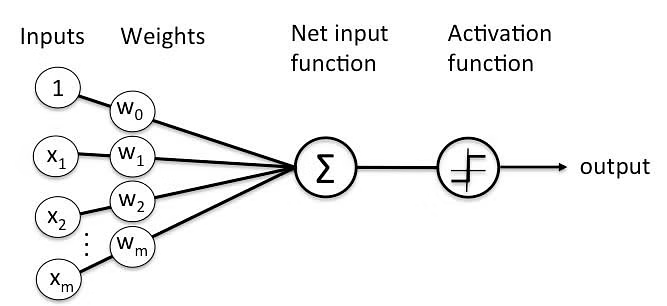
\includegraphics[width=0.6\linewidth]{perceptron.png}
	\caption[Illustration d'un perceptron]{Illustration d'un perceptron. Source : \cite{PerceptronImage}}
\end{figure}

Les paramètres d'un perceptron sont : un bias, et $x$ données d'entrées avec des poids associés. Toutes ces valeurs pondérées sont ensuite additionnées ensemble
et passées à une fonction d'activation qui donnera la valeur finale de sortie au perceptron. En général la fonction d'activation est une sigmoïde, 
mais pourrait être n'importe quelle fonction mathématique qui s'adapterai mieux au problème que l'on essaye de résoudre.

Avec un seul perceptron, il est possible d'ajuster ces poids de telle manière à lui faire apprendre une motif de
séparation linéaire en fonction des données d'entrée. 

\begin{figure}[tbph!]
	\centering
	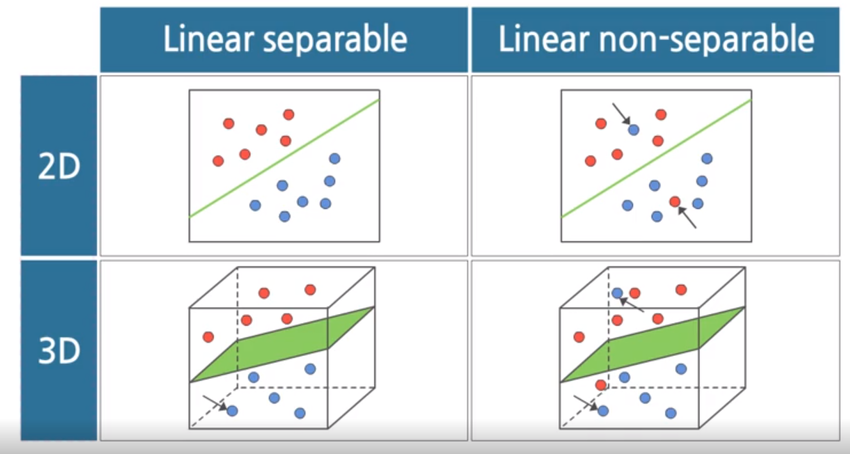
\includegraphics[width=0.4\linewidth]{separation-lineaire.png}
	\caption[Comparaison de données séparables ou non linéairement]{Comparaison de données séparables ou non linéairement. Source : \cite{LinearSeparation}}
\end{figure}

Il a donc été rapidement imaginé d'interconnecter ces perceptrons pour permettre d'apprendre des problèmes non linéaires. 
Créant l'architecture la plus simple le "Multi Layer Perceptron" ou perceptron multi-couches.

\subsection{Multi Layer Perceptron}

Cette architecture de réseaux de neurones consiste simplement à créer 3 types de couches avec un nombre variable de perceptron pour chacune d'entre-elles :

\begin{figure}[tbph!]
	\centering
	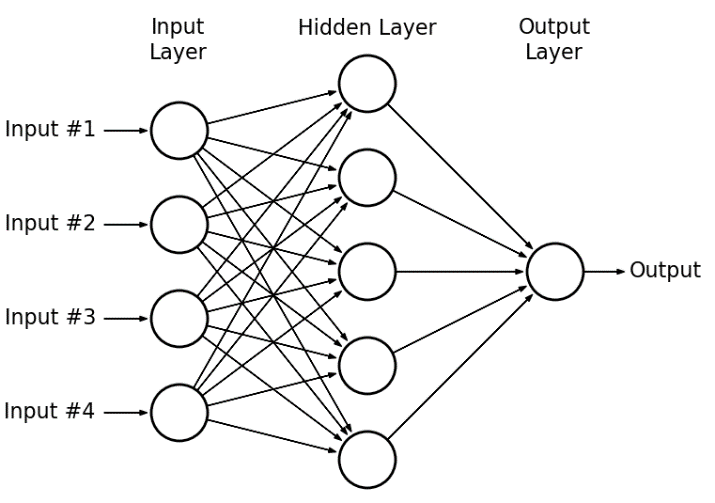
\includegraphics[width=0.4\linewidth]{MLP.png}
	\caption[Exemple d'un perceptron multi-couches]{Exemple d'un perceptron multi-couches. Source : \cite{MLPImage}}
\end{figure}

\begin{itemize}
	\item 1 couche d'entrée : Cette couche représente seulement les valeurs d'entrées de manière organisée, 
	par exemple une image de 10x10 pixels aurait une couche de taille 100. 
	\item $x$ nombre de couches cachées : Ici un nombre de couches indéterminées peuvent être ajoutées. 
	Chacune d'entre elles ont peuvent avoir un nombre de neurones différents dépendant du problème à traiter. d'analyser les 
	\item 1 couche de sortie : Cette couche peut aussi avoir une taille variable deépendant de ce que le modèle doit accomplir. 
	Par exemple si le modèle à comme but de détecter si une image est un chat ou non cette couche pourrait n'avoir qu'un neurone avec une fonction d'activation sigmoïde.
\end{itemize}

Entre chacune de ces couches, chaque neurone est connecté avec chacun des autres de la couche suivante, créeant des couches surnommées "denses".

\subsection{Apprentissage}

Peu importe le nombre de couches ou de neurones qui composent un réseau, il faut bien que celui-ci aprenne à résoudre le problème pour lequel il a été conçu.
Cet apprentissage se repose sur les bases mathématiques que le perceptron utilise. 
Lorsque l'on calcule le résultat d'un perceptron celui-ci va en calculer une ou plusieurs valeurs en sortie.
Lors d'un apprentissage supervisé, les valeurs de sortie attendues sont connues. On peut en calculer une valeur d'erreur avec une fonction mathématique.
Nous avons donc volonté dans ce cas de minimiser cette fonction d'erreur. Et il est possible de le faire en modifiant les poids des valeurs d'entrées. 
La manière de trouver comment modifier ces poids s'apelle la descente de gradient.

\begin{figure}[tbph!]
	\centering
	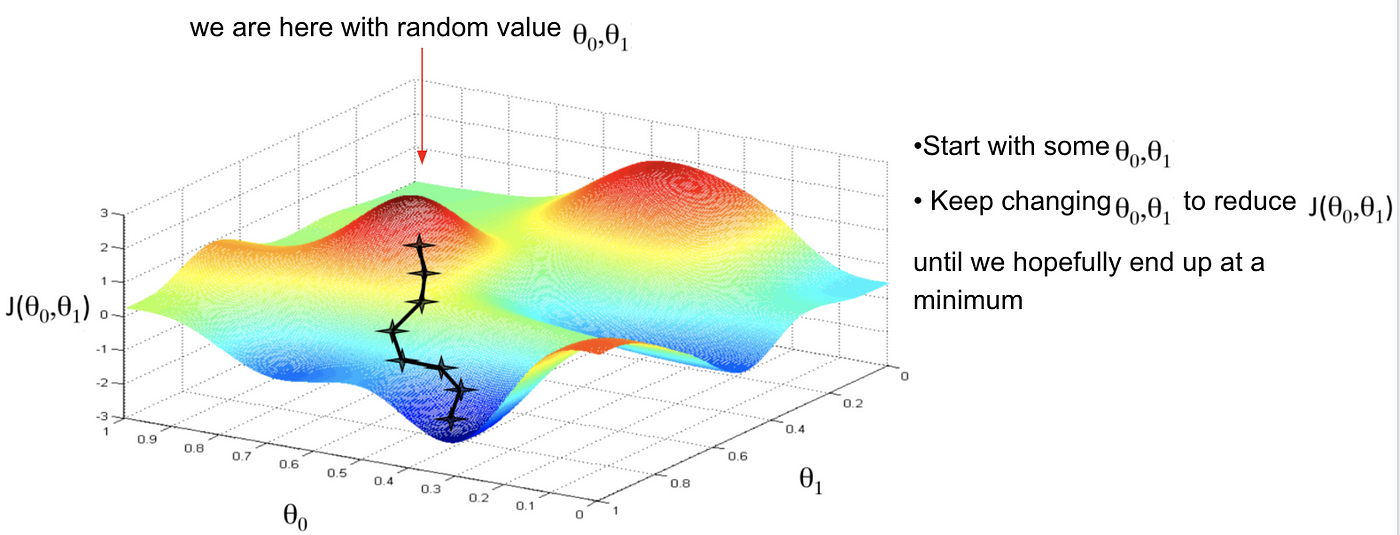
\includegraphics[width=0.8\linewidth]{gradient_descent.png}
	\caption[Exemple d'une descente de gradient en 3D]{Exemple d'une descente de gradient en 3D. Source : \cite{GradientDescentImage}}
\end{figure}

Il est donc possible de trouver comment modifier les valeurs de chaque poids ou bias
de chaque neurones afin de minimiser la fonction d'erreur et cela s'appelle la "backward propagation error" ou
"backpropagation".

Un piège fréquent lors de l'entraînement de réseaux neuronaux est l'overfitting. Le processus d'apprentissage fonctionne parfois trop "bien"
su les données utilisées, jusqu'au point ou le réseau de neurones à trouver des correspondances ou des motifs qui ne sont pas ceux que l'on recherche.
Le rendant hyper spécifié à nos données d'entraînement uniquement.

Par exemple, pour un réseau essayant de différencier des images de chaussures d'autres vêtements. Si, malheureusement, toutes les chaussures sont vertes,
le réseau pourrait en déduire que c'est la couleur qui permet de les différencier. Cependant, lorsque le modèle sera présenté 
une chaussure rouge qui ne faisait pas partie des données d'entraînement celui-ci ne la reconnaitra pas.

\subsection{Réseau de neurones convolutif}

Comme évoqué précedemment, il existe une infinité d'autres configuration pour un réseau de neurones, alors nous ne regarderons en détails 
que les différentes configurations qui ont été envisagées dans ce projet.

L'une des premières architecture de réseau neuronal qui a été envisagée pour ce projet à été le réseau de neurones convolutif.
Celui-ci consiste à certaines couches cachées d'une manière spécifique qui effectuera le même calcul qu'une convolution.

\begin{figure}[tbph!]
	\centering
	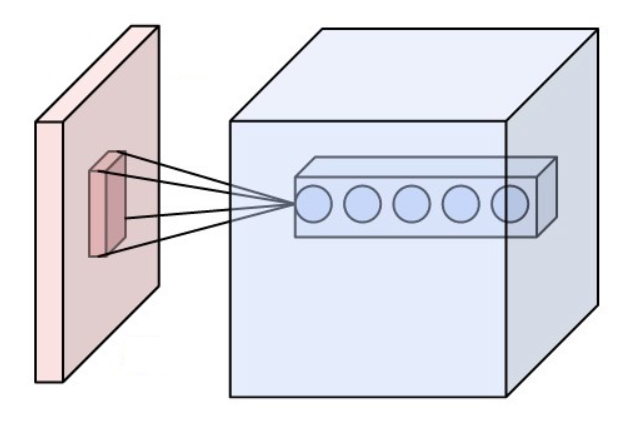
\includegraphics[width=0.4\linewidth]{Conv_layer.png}
	\caption[Illustration d'une couche convolutive de réseau neuronal]{Illustration d'une couche convolutive de réseau neuronal. Source : \cite{ConvImage}}
\end{figure}

L'opération de convolution en mathématique permet généralement d'extraire des informations d'une image comme le taux de 
variation d'intensité entre chaque pixel lors d'une détection de contours par exemple.
Ici, la différence est que le noyau utilisé pour la convolution n'est pas un noyau provenant d'algorithmes comme Sobel ou Canny mais ce sera
l'apprentissage du réseau qui va établir un noyau le plus optimisé pour trouver les caractéristiques recherchées dans les données d'entrée.

\subsection{Réseau de neurones récurrents}

Un autre type de réseau neuronal est le réseau de neurones récurrents. Cette architecture est adaptée
à des problèmes comprenant des données séquentielles ou temporelles généralement comme de la détection automatique de parole ou de texte.

Cette architecture diffère des autres réseaux de neurones car elle contient un mécanisme de "mémoire" intégré dans le modèle.
La mémoire est généralement implémentée en connectant sortie du premier neurones comme une entrée supplémentaire a la couche cachée du deuxième neurone.

\begin{figure}[tbph!]
	\centering
	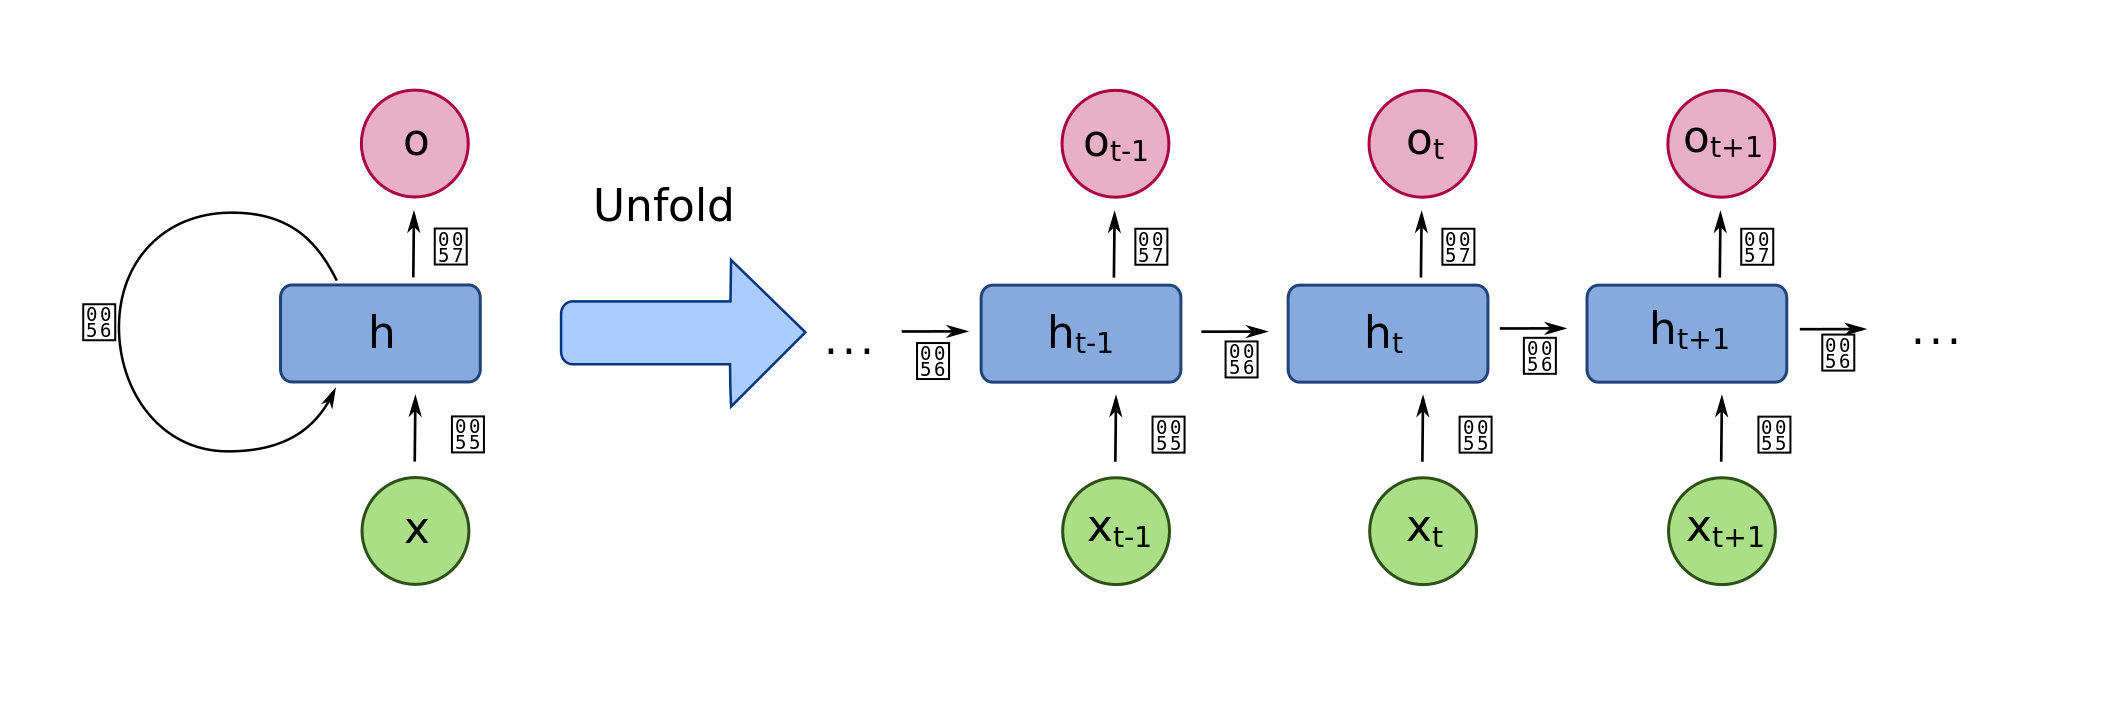
\includegraphics[width=0.8\linewidth]{rnn.png}
	\caption[Illustration de réseau de neurones récurrents]{Illustration de réseau de neurones récurrents. Source : \cite{RnnImage}}
\end{figure}

Cette "mémoire" n'existe donc que de manière temporaire à chaque exécution du réseau. Certains autres configuration comme les LSTM pour "Long and Short Term Memory"
sont aussi capable de se souvenir sur un plus long terme.

\subsection{Auto-encodeurs}

Lors de la première partie de ce projet se focalisant sur les problématiques du télescope Terzina, un autre type de réseau 
avait été envisagé pour sa capacité à compresser des données : les auto-encodeurs.

L'auto-encodeur est une architecture de réseau de neurones particulière qui comprend deux parties distinctes d'encodage et de décodage. 
Ces deux étapes peuvent aussi être perçues comme une compression et décompression successive. \cite{IbmAutoencoder}

\begin{figure}[tbph!]
	\centering
	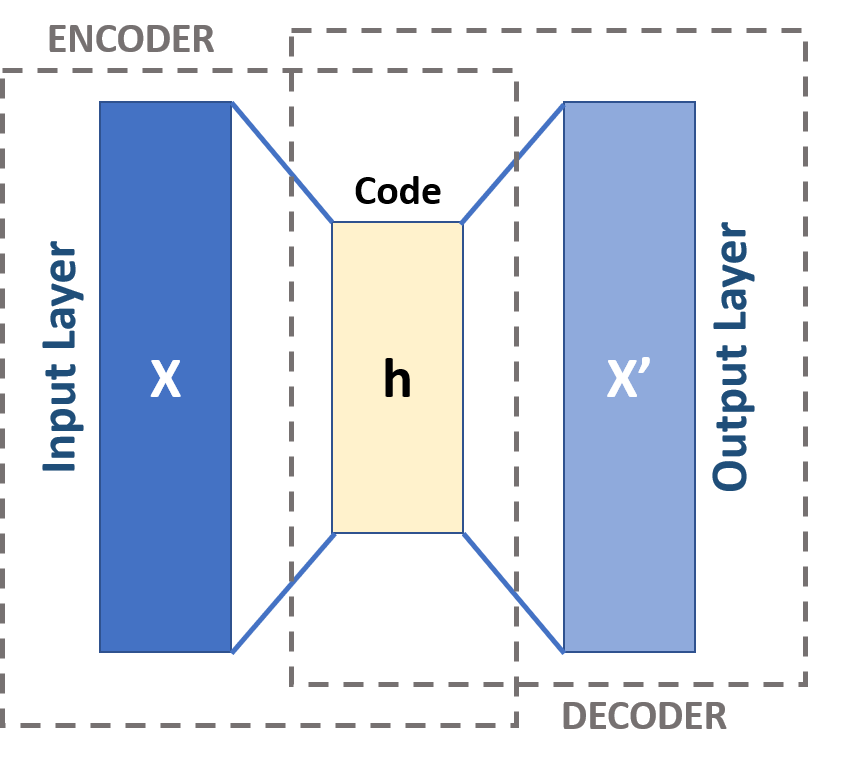
\includegraphics[width=0.4\linewidth]{Autoencoder.png}
	\caption[Schéma d'auto-encodeur]{Schéma d'auto-encodeur. Source : \cite{Autoencoder}}
\end{figure}

En entraînant le réseau de neurones, celui-ci va apprendre à réduire les informations en entrée jusqu'à un minimum pour 
ensuite essayer de reproduire au mieux les données originales à partir de cette représentation réduite.
Ceci résulte en général en une perte de précision des données lors de la compression.

\subsection{Couches}
Les configurations vues jusqu'à maintenant peuvent aussi être combinées entre elles pour former de plus grand réseaux de neurones.
Les réseaux neuronaux peuvent donc avoir une partie de réseau CNN et RNN, etc. Chacune des couche peut-ainsi être catégorisée par
rapport à sont utilité.
Il existe aussi plus de couches spécifiques capable de travail spécifique. En voici plusieurs utilisées au cours de ce travail ainsi que leur utilité :

\subsubsection{BatchNormalisation}
La couche "BatchNormalisation", en général utilisée en premier dans un réseau, sert à normaliser les données qui lui sont données.
Cela sert à généraliser le reste du traitement du réseau, par exemple si l'on traitait des images avec des expositions différentes.

\subsubsection{Flatten}
Lors de l'utilisation de couches de convolution, il est possible d'en effectuer plusieurs en même temps et de les traiter parallèlement.
On peut ensuite utiliser une couche "Flatten" pour rassembler ces données en une seule dimension.

\subsubsection{Pooling}
Ce type de couche dans un réseau neuronal permet de réduire le nombre de dimensions qui lui sont données en entrées.
Ses utilités sont de réduire la quantité de calculs suivant cette couche et réduit l'overfitting lors de l'entraînement.

Les deux manières les plus communes pour effectuer un pooling est de garder la moyenne ou le maximum de chaque dimension :

\begin{figure}[tbph!]
	\centering
	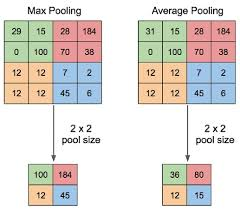
\includegraphics[width=0.4\linewidth]{pooling_layers.jpeg}
	\caption[Illustration du principe de Pooling]{Illustration du principe de Pooling. Source : \cite{PoolingImage}}
\end{figure}

\subsubsection{Dropout}
Cette couche sert une même utilité que le Pooling en réduisant le nombre d'entrées qui sont passés à la suite du réseau afin d'en réduire l'overfitting.
Cependant, ici il ne s'agit pas de transformation au niveau des dimensions mais une simple gestion de pourcentage qui sera gardée/épurée.

\section{Données}

Une autre grande partie de ce projet à été la gestion des données utilisées pour tester les différents réseaux de neurones.

\subsection{Pe Extractor}

Le premier simulateur qui a été fourni provenait d'un projet existant de l'\gls{unige} s'appelant "pe\_extractor".
Ce projet Python contient un générateur de signal avec du bruit NSB dans lequel des photon-électron sont insérés.
Le concept de photon-électron ou \gls{pe} est l'interaction physique lorsqu'un photon est détecté par un capteur et converti en charge électromagnétique analogique.
Cette quantité électromagnétique est appelée photon-électron.

Le bruit NSB pour un télescope est le bruit de fond minimum lorsqu'il pointe le ciel pendant la nuit. Même dans ces meilleurs condition,
de la lumière provenant des villes et de l'atmosphère est détectée par le télescope. 
De manière aléatoire et selon une fréquence donnée, le générateur ajoute au signal l'amplitude simulée d'un photon-électron.
Cette amplitude est définie par un fichier d'impulsion qui dépend du capteur utilisé.

Le générateur fournis deux tableaux en sortie : le signal discrétisé et des bacs contenant la vérité du nombre de \gls{pe} ayant été injectés sur cette période.

Voici les paramètres importants du générateur et leur explication :
\begin{enumerate}
    \item "pe\_rate\_mhz" : Définit la fréquence moyenne à laquelle un \gls{pe} est injecté dans le signal.
        L'injection de \gls{pe} est aléatoire en suivant une distribution Poisson.
    \item "sampling\_rate\_mhz" : Définit la vitesse d'échantillonnage du signal. Pour Terzina, cela est de 200MHz.
    \item "n\_sample" et "n\_sample\_init" : Le générateur a un mécanisme d'initialisation pour le bruit électrique 
        qui peut prendre un certain nombre de cycles pour commencer a créer des informations cohérentes au niveau physique, 
        ces deux paramètres peuvent donc contrôler un nombre d'échantillons à écarter au début de la génération.
    \item "bin\_size\_ns" : Ce paramètre gère la période de comptabilisation des \gls{pe} insérés dans le signal de sortie.
    \item "shift\_proba\_bin" : Permet de décaler la comptabilisation de l'insertion de signal par un certain nombre de bacs.
        Ce système existe car l'impulsion a un temps de montée avant d'atteindre son pic, cela permet de décaler les bacs 
        de vérité pour s'aligner avec le pic de l'impulsion.
    \item "sigma\_smooth\_pe\_ns" : Ce paramètre sert à répartir le compte des \gls{pe} insérés sur les bacs voisines en ns
        pour éviter une vérité entière. 
    \item "noise\_lsb" : Est une quantité de bruit électronique.
\end{enumerate}

Les bacs contenant les photons insérés dans le signal bruité à une meilleure résolution que le signal discrétisé. 
Une première adaptation a été programmée pour regroupper ces bacs sur la même fréquence d'échantillonage du signal :

\begin{figure}[tbph!]
	\centering
	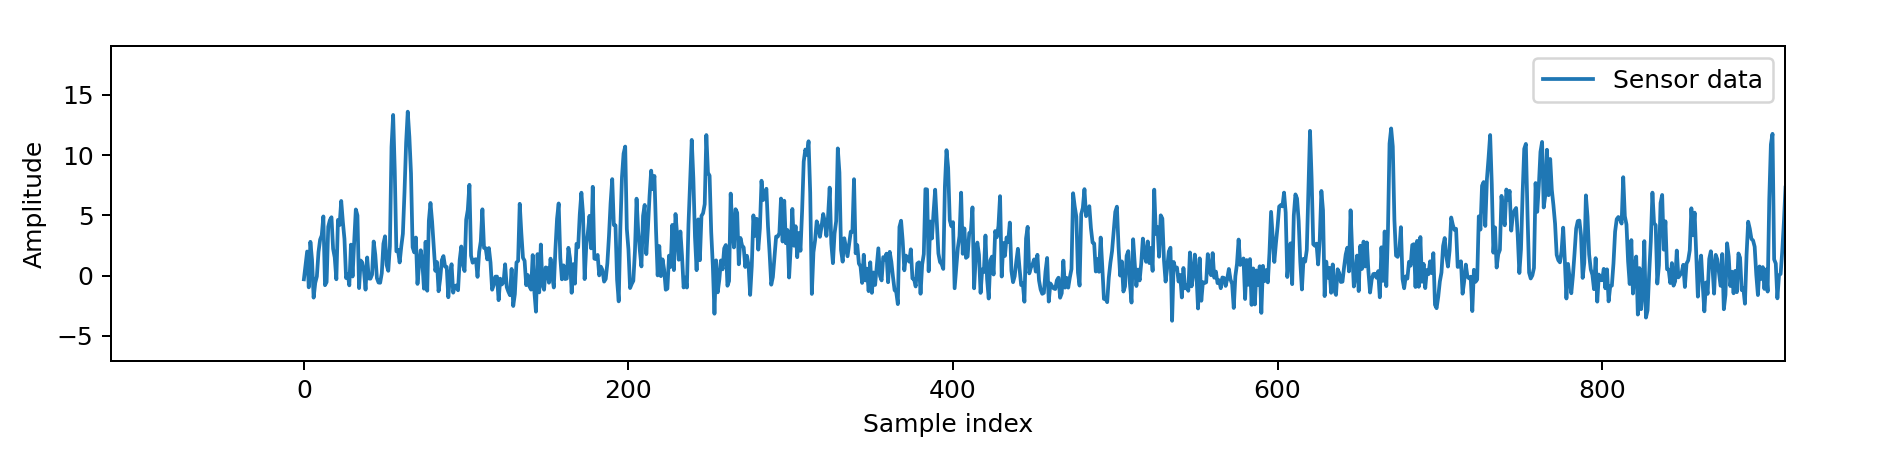
\includegraphics[width=\linewidth]{sensor_waveform.png}
	\caption[Exemple de signal simulé]{Exemple de signal simulé.}
\end{figure}

\subsection{Fichiers de simulation Corsika}

Le premier simulateur de signal provenant de "pe\_extractor" ne simule que des interférences de type NSB. 
Pour se rapprocher des données réelles des caméras, il a été choisi de récupérer des fichiers de simulation de pluies Cherenkov pour le \gls{lst}.

Ces fichiers de simulations contiennent énormément de données, de la configuration du télescope, jusqu'au impact des photons provenant des pluies Cherenkov.
Ceux-ci sont stockés sur le partage de fichiers du cluster Yggdrasil de l'\gls{unige} sous un format de fichier ROOT. 

ROOT est un framework logicel conçu par le \gls{cern} pour l'analyse de données et la gestion d'entrées et sorties. Ces types de fichiers
sont souvents utilisés pour stocker de manière structurée des données provenant d'expériences scientifiques en tant qu'arbres et tableaux
pour réduire l'espace de stockage utilisé par un ficher.

Ces différentes données ne sont pas utilisables directement et doivent être réinterprétées par le logiciel "pyeventio\_example" aussi fournis
par l'équipe de l'\gls{unige}. Ce projet met à disposition un exécutable nommé "runana" qui permet de recréer un fichier binaire 
contenant certaines métadonnées, le signal de chaque capteur composant la caméra du télescope et les instants auxquels les photons 
provenant de la pluie Cherenkov ont impactés le capteurs.

% \section{Outils}
% \subsection{Tensorflow}
% \subsection{Keras}